\documentclass[a4paper,12pt]{article}
\usepackage[margin=2cm]{geometry}
\usepackage[czech]{babel}
\usepackage[utf8]{inputenc}
\usepackage{amsmath}
\usepackage{amssymb}
\usepackage{graphicx}
\usepackage{fancyhdr}
\usepackage{lipsum}
\usepackage[backend=bibtex,sorting=none]{biblatex}
\usepackage{tikz}

\usetikzlibrary{shapes.geometric, arrows}
\tikzstyle{block} = [rectangle, minimum width=3cm, minimum height=1cm,text centered, draw=black, fill=gray!25]
\tikzstyle{arrow} = [thick,->,>=stealth]
\addbibresource{ZMP.bib}

\def\max #1{\textrm{max}\left\{#1\right\}}
\def\CS{C\texttt{\#}}
\renewcommand{\labelitemii}{$\circ$}
\renewcommand{\labelitemiii}{$-$}
\makeatletter
\newcount\my@repeat@count
\newcommand{\repeatchar}[2]{%
  \begingroup
  \my@repeat@count=\z@
  \@whilenum\my@repeat@count<#1\do{#2\advance\my@repeat@count\@ne}%
  \endgroup
}
\makeatother

\author{Richard Blažek}
\setlength{\headheight}{15pt}
\pagestyle{fancy}
\fancyhead{}
\fancyhead[R]{Imperit}
\fancyhead[L]{Richard Blažek}
\fancyfoot{}
\fancyfoot[R]{\thepage}
\fancyfoot[L]{Kapitola \thesection}
\setlength{\parindent}{0pt}
\setlength{\parskip}{0.8em}

\begin{document}
\begin{titlepage}
    \begin{center}

	\vspace*{3cm}            
	\Huge
	\textbf{Imperit}
            
	\vspace{0.5cm}
	\LARGE
	Strategická tahová hra
        
	\vspace*{1cm}
	\Huge
	\textbf{Imperit}
            
	\vspace{0.5cm}
	\LARGE
	Turn-based strategy
            
	\vfill
            
	\large
        Závěrečná maturitní práce, rok 2021\\
	Richard Blažek\\
	Gymnázium Brno, třída Kapitána Jaroše 14
    \end{center}
\end{titlepage}
\thispagestyle{empty}
\Large\textbf{Prohlášení}\normalsize

Prohlašuji, že jsem svou závěrečnou maturitní práci vypracoval samostatně a použil jsem pouze prameny a literaturu uvedené v seznamu bibliografických záznamů.

Prohlašuji, že tištěná verze a elektronická verze závěrečné maturitní práce jsou shodné.

Nemám závažný důvod proti zpřístupňování této práce v souladu se zákonem č. 121/2000 Sb., o právu autorském, o právech souvisejících s právem autorským a o změně některých zákonů (autorský zákon) ve znění pozdějších předpisů. 

V Brně dne \today{} \repeatchar{40}{.}
\newpage
\thispagestyle{empty}
\Large\textbf{Poděkování}\normalsize

Tímto bych chtěl poděkovat Mgr. Marku Blahovi za odborné vedení práce.
\newpage
\thispagestyle{empty}
\Large\textbf{Anotace}\normalsize

Práce se zabývá vytvořením internetové počítačové hry zvané Imperit pomocí Blazor WebAssembly z frameworku .NET. Hra je koncipovaná jako tahová strategie, jejímž tématem je dobývání území na herním plánu, s právě jedním vítězem a omezeným náhodným prvkem.

\Large\textbf{Klíčová slova}\normalsize

počítačová hra;tahová strategie;blazor;webassembly;dotnet;hra s nulovým součtem;územní expanze

\Large\textbf{Annotation}\normalsize

The thesis is concerned about creation of online browser-based game called Imperit using Blazor WebAssembly from the .NET framework. The game is designed as a turn-based strategy consisting of conquering the territory on the game map, having exactly one winner and a limited element of chance.

\Large\textbf{Keywords}\normalsize

computer game;turn-based strategy;blazor;webassembly;dotnet;zero-sum game;territorial expansion
\newpage
\thispagestyle{empty}
\tableofcontents
\newpage
\section{Úvod}
Rozhodl jsem se vytvořit hru o dobývání území navrženou tak, aby byla konečná a vítěz byl jednoznačně určen. Vítězství by však nemělo na konci hry nastat neočekávaně, již v průběhu hry bude patrný vývoj, z něhož vyplyne, který hráč má k výhře nejblíže, ale tento vývoj budou moci ostatní hráči zvrátit. Hra by také měla obsahovat náhodný prvek, ovšem pravděpodobnost náhodných jevů by měla být známá, aby byli hráči nuceni s rizikem počítat.

Pro vytvoření hry jsem zvolil formát tahové strategie, neboť strategie v reálném čase buď vyvíjí tlak na hráče z důvodu nedostatku času, nebo ve snaze vyhnout se tomuto problému vede ke zdlouhavému čekání na dokončení některých akcí \cite{turnreal1}. V obou případech realtimová strategie vede k orientaci na postřeh a trpělivost spíše než na vymýšlení strategie\cite{turnreal2}. Kromě toho \uv{připoutává} hráče k jejich obrazovkám, což sice může být mnohdy žádoucí, ale můj záměr takový nebyl.

\section{Popis hry}
\subsection{Provincie}
Hra se odehrává na plánu, který se skládá z provincií (země, moře a pohoří), jejichž názvy a tvary jsou zvolené podle evropských zemí a moří nebo jejich části. Provincie obsahují vojenské jednotky a jsou ovládány nejvýše jedním hráčem, který v nich může verbovat jednotky. Země se mohou odtrhnout a pravděpodobnost, že se tak v daném kole stane je $P=\max{\displaystyle\frac{P_0\cdot (S_0-S)}{S_0},0}$, kde $P_0$ je výchozí pravděpodobnost odtržení (příbližně 10 \%), $S$ je obranná síla jednotek přítomných v zemi a $S_0$ je obranná síla výchozích jednotek, jež byly v zemi na začátku hry. Provincie je dobyta, je-li napadena vojskem, jehož útočná síla je vyšší, než je obranná síla jednotek v provincii. V zemích označených kotvou jsou přístavy, které umožňují přesun na moře a z moře.
\subsection{Hráči}
Hráčů může být $2$--$16$. Při registraci si zvolí zemi, v níž budou začínat, a na začátku hry dostanou určité množství peněz. Dále získají v každém kole určité množství peněz za každou zemi, kterou ovládají, přičemž toto množství se u různých zemí liší. Za peníze si mohou kupovat země a verbovat ve svých provinciích vojenské jednotky.
\subsection{Vojenské jednotky}
Vojenské jednotky slouží k dobývání provincií. Každá jednotka má určitou cenu, sílu v obraně, sílu v útoku a hmotnost, jež je relevantní v případě, že jednotka nemůže provést určitý přesun samotná a potřebuje například loď k přesunu přes moře. Jednotky schopné přenášet jiné (např. loď, slon) mají též nosnost, jež udává, jaká může být celková hmotnost jednotek, které se s ní přepravují.
\subsection{Začátek}
Při registraci si hráč zvolí jméno a heslo a zobrazí se mu mapa, na níž si může vybrat zemi, v níž bude začínat. Tato mapa vypadá stejně jako mapa popisovaná v sekci 2.7.1, ale názvy provincií, v nichž není možné začínat jsou napsány šedě. Po registraci musí počkat, až začne jeho hra. Hra začne čtyři minuty po registraci druhého hráče, aby žádný hráč nemusel dlouho čekat, ale aby každý měl nějakého lidského protihráče.
\subsection{Průběh hry}
Tahy hráčů se střídají v tom pořadí, v němž se tito hráči zaregistrovali. Během tahu je možné provést neomezené množství akcí bez časového limitu. Mezi akce se řadí verbování, přesun armády, koupě provincie, věnování peněz jinému hráči a kapitulace. Verbování a přesun se dokončí až po konci hráčova tahu, ostatní akce proběhnou okamžitě.
\subsection{Cíl hry}
Cílem hry je ovládnout tři ze čtyř cílových provincií, které jsou rozprostřeny po všech okrajích mapy, takže k dobytí všech je nutné ovládnout podstatnou část mapy. Zvolí-li však hráč vhodnou strategii, může vyhrát, aniž by měl největší území.
\subsection{Ovládání}
Hráč má na okraji (levý okraj na širokých obrazovkách, horní na úzkých) má navigační menu, v němž může přepínat mezi stránkami. Při přihlášení se jako výchozí stránka zobrazuje mapa provincií.
\subsubsection{Mapa}
Na této stránce hráč vidí mapu všech provincií. Pohoří se zobrazují jen jako šedá čára mezi zeměmi. Pokud jim žádný z hráčů nevládne, jsou moře tyrkysová a země černošedé; pokud v nich však někdo vládne, mají barvu onoho hráče. Dále se u nich zobrazuje jejich název a počet vojenských jednotek v nich, u zemí se navíc zobrazuje jejich výnos za jedno kolo. Země, které mají přístav, mají u svého názvu kotvu, a země, které hráč potřebuje k vítězství, u svého názvu mají hvězdičku.

Klikne-li hráč dvakrát na svou provincii, může v ní verbovat jednotky; klikne-li na ni jednou a poté klikne na druhou provincii, může přesunout jednotky z první provincie do druhé; klikne-li na cizí zemi, jež sousedí s jeho zemí, může tuto zemi koupit. Při verbování (resp. přesunu) se ukáže nabídka, v níž může hráč vybrat, kolik jednotek kterého druhu chce verbovat (resp. přesunout). Pokud se hráč rozhodne verbovat více jednotek, než si může za své peníze koupit, nebo si koupit zemi, která stojí více peněz, než kolik daný hráč má, zobrazí se mu možnost si chybějící částku půjčit. Pokud se země může odtrhnout, zobrazí se v nabídce verbování pravděpodobnost, že k tomu dojde.

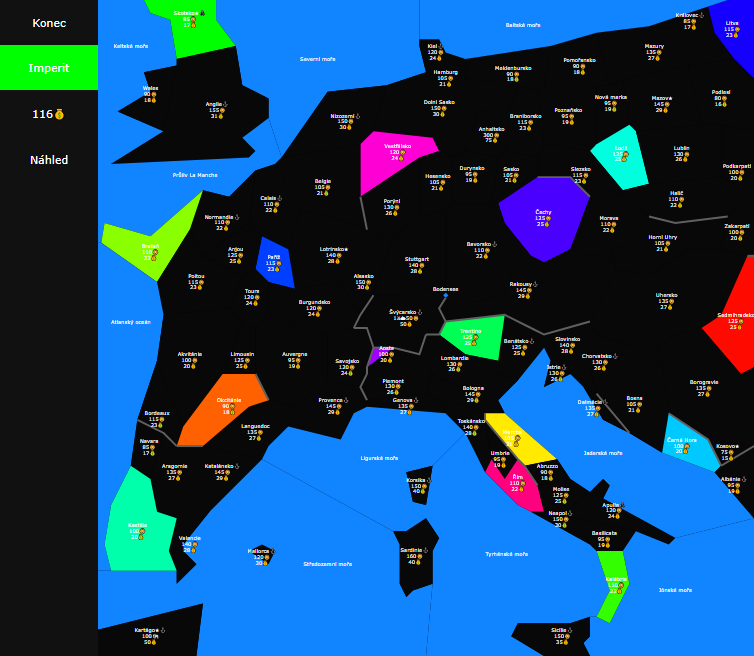
\includegraphics[width=\textwidth]{ProvinceMap.png}

Navigační menu na této stránce má čtyři položky. První z nich je konec tahu, nebo odhlášení, podle toho, zda je přihlášený hráč na tahu. Druhá položka pouze informuje o tom, kolik peněz má přihlášený hráč. Třetí položka přepíná na stránku \textit{Hráči} a poslední možnost ukazuje náhled mapy po provedení akcí hráče na tahu.
\subsubsection{Hráči}
Na této stránce se zobrazuje seznam všech hráčů, jejich peníze, příjmy, případě výše jejich dluhů. Klikne-li hráč na jméno jiného hráče, může mu věnovat peníze. Zobrazí se nabídka a v ní lze vybrat, kolik peněz darovat. Pod seznamem hráčů je možnost vzdát se, kliknutím na ni hráč zemře a všechny jeho provincie se odtrhnou.

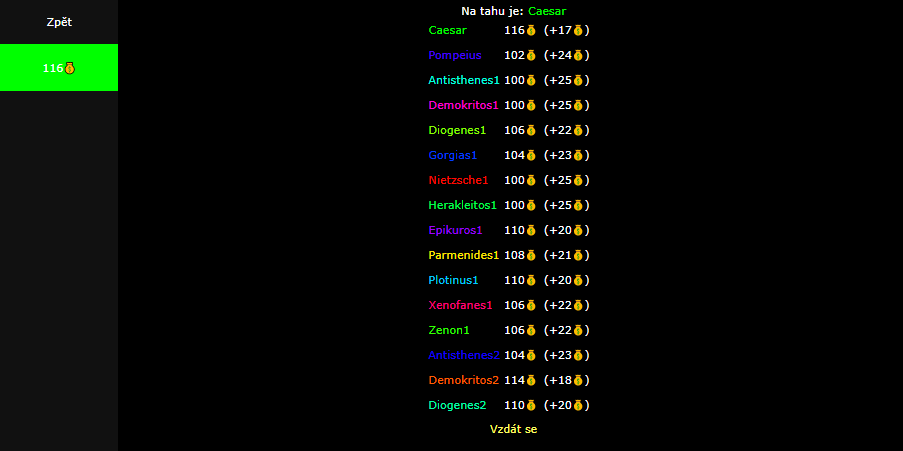
\includegraphics[width=\textwidth]{Players.png}

Pokud hra trvá dostatečně dlouho, zobrazí se pod možností vzdát se tři grafy. První z nich popisuje vývoj celkových sil hráčů (počítají se jako součet ceny všech vojáků, peněz, pětinásobku příjmů a stonásobku počtu cílových zemí, které daný hráč vlastní). Na druhém grafu se zobrazuje poměrná změna této síly. Na třetím se zobrazuje poměr vojenských sil hráčů (počítají se jako součet ceny všech vojáků a peněz) vůči sobě.

\section{Použité technologie}
\subsection{\CS{}}
Celý program je napsaný v jazyce \CS{}, neboť tento jazyk může běžet na straně serveru (viz ASP.NET Core) i klienta (viz Blazor WebAssembly) a obě části mohou využívat společné knihovny a pracovat s týmiž datovými typy. Navíc tento jazyk umožňuje využívat knihoven z frameworku .NET a na rozdíl od jazyků PHP a JavaScript, které se často pro vývoj webových aplikací používají, je staticky typovaný a kompilovaný do bytekódu, což do určité míry kontroluje správnost programu.
\subsection{ASP.NET Core}
Framework ASP.NET Core je využíván na straně serveru ke zpracovávání HTTP dotazů a odesílání odpovědí.
\subsection{Blazor WebAssembly}
Blazor WebAssembly je framework, který umožňuje vyvíjet v jazyce  \CS{} aplikace spustitelné v prohlížeči. Kód v jazyce  \CS{} se přeloží do binárního formátu WebAssembly a prohlížeč pomocí krátkého kódu v JavaScriptu výsledný soubor stáhne a spustí. Spuštěný program následně reaguje na akce uživatele, komunikuje se serverem pomocí HTTP a podle potřeby překresluje zobrazovanou webovou stránku.

\section{Struktura}
Program se skládá ze tří projektů:
\begin{itemize}
\item\textit{Shared} -- Obsahuje třídy, které druhé dva projekty využívají, nachází se v něm většina herní logiky a odpovídá větší části modelu v architektuře MVC\cite{mvc}
\item\textit{Client} -- Odpovídá pohledu v architektuře MVC a obsahuje soubory v HTML, CSS a kód v  \CS{}, překládaný do WebAssembly a spouštěný v prohlížeči klienta
\item\textit{Server} -- Zahrnuje kód spouštěný na straně serveru, což znamená zejména práci s databází a webové API, které odesílá odpovědi na dotazy klienta; v architektuře MVC odpovídá kontroleru a části modelu
\end{itemize}
\begin{tikzpicture}[node distance=2cm]
\node (shared) [block] {Shared};
\node (client) [block, right of=shared, xshift=2cm] {Client};
\node (server) [block, below of=shared] {Server};
\draw [arrow] (client) -- (shared);
\draw [arrow] (server) -- (shared);
\draw [arrow] (server) -- (client);
\end{tikzpicture}
\newpage
\printbibliography[heading=bibintoc, title={Použitá literatura}]
\end{document}